\section{Experiments}
\label{sec:expr}

Based on LSH, LSB \cite{lsb}, and DSH\footnote{We implement DSH by ourselves because it is not public available.}, we implement LayerLSH, LayerLSB, and LayerDSH respectively.  The experiments were performed on a Ubuntu system equipped with one Intel(R) Xeon(R) 2.60GHz CPU, 32GB of memory.

\Paragraph{Datasets and Queries} We evaluate our approach using six real datasets, including \textbf{KDD}\footnote{http://www.kdd.org/kdd-cup/view/kdd-cup-2004/Data}, \textbf{Forest}\footnote{http://archive.ics.uci.edu/ml/datasets/Covertype}, \textbf{Color}\footnote{http://kdd.ics.uci.edu/databases/CorelFeatures/}, \textbf{Audio}\footnote{http://www.cs.princeton.edu/cass/audio.tar.gz}, and \textbf{Mnist}\footnote{http://yann.lecun.com/exdb/mnist/}. Properties of these three datasets are summarized in Table \ref{tab:data}. We also generate three sets of queries from each dataset. We first evaluate the density of each point, which is the number of neighbors in a given radius, then extract the top 2\% highest density points as \textbf{dense queries}, the top 2\% lowest density points as \textbf{sparse queries}, and the randomly sampled 2\% points as \textbf{random queries}.

%These real datasets exhibit various skewness. The skewness is captured by the variability of point densities. We show the 10th percentile, the 50th percentile and the98th percentile of the point densities for these datasets. The greater variation of these percentiles indicates a more skewed data distribution.

\begin{table}[!htb]
\vspace{-0.1in}
    \caption{Datasets}
    \vspace{-0.15in}
    \label{tab:data}
    \centering
    \small
    \begin{tabular}{c|c|c|c}
    \hline
   data & instances & dim & size\\
\hline\hline
KDD & 145,751 & 75 & 33MB\\
\hline
Forest & 581,012 & 55 & 77MB \\
\hline
Color & 68,040 & 32 & 10MB \\
\hline
Audio & 54,387 & 192 & 36MB\\
\hline
Mnist & 60,000 & 256 & 41MB\\
\hline
\end{tabular}
\vspace{-0.1in}
\end{table}

\begin{figure*}[!t]
\vspace{-0.2in}
	\centerline{
	\subfloat[KDD]{\includegraphics[angle=-90, width=1.6in]{fig/lsh_kdd.eps}
    \label{fig:ratio:kdd}
    \vspace{-0.05in}}
    \hspace{-5mm}
    \subfloat[Forest]{\includegraphics[angle=-90, width=1.6in]{fig/lsh_forest.eps}
    \label{fig:ratio:forest}
    \vspace{-0.05in}}
    \hspace{-5mm}
    \subfloat[Color]{\includegraphics[angle=-90, width=1.6in]{fig/lsh_color.eps}
    \label{fig:ratio:color}
    \vspace{-0.05in}}	
    \hspace{-5mm}
    \subfloat[Audio]{\includegraphics[angle=-90, width=1.6in]{fig/lsh_audio.eps}
    \label{fig:ratio:audio}
    \vspace{-0.05in}}
    \hspace{-5mm}
    \subfloat[Mnist]{\includegraphics[angle=-90, width=1.6in]{fig/lsh_mnist.eps}
    \label{fig:ratio:mnist}
    \vspace{-0.1in}}
    }
    \vspace{-0.1in}
	\caption{LSH vs. LayerLSH.}
	\label{fig:lshresult}
\vspace{-0.1in}
\end{figure*}

\begin{figure*}[!t]
\vspace{-0.1in}
	\centerline{
	\subfloat[KDD]{\includegraphics[angle=-90, width=1.6in]{fig/lsb_kdd.eps}
    \label{fig:lsb:kdd}
    \vspace{-0.05in}}
    \hspace{-5mm}
    \subfloat[Forest]{\includegraphics[angle=-90, width=1.6in]{fig/lsb_forest.eps}
    \label{fig:lsb:forest}
    \vspace{-0.05in}}
    \hspace{-5mm}
    \subfloat[Color]{\includegraphics[angle=-90, width=1.6in]{fig/lsb_color.eps}
    \label{fig:lsb:color}
    \vspace{-0.05in}}	
    \hspace{-5mm}
    \subfloat[Audio]{\includegraphics[angle=-90, width=1.6in]{fig/lsb_audio.eps}
    \label{fig:lsb:audio}
    \vspace{-0.05in}}
    \hspace{-5mm}
    \subfloat[Mnist]{\includegraphics[angle=-90, width=1.6in]{fig/lsb_mnist.eps}
    \label{fig:lsb:mnist}
    \vspace{-0.1in}}
    }
    \vspace{-0.1in}
	\caption{LSB vs. LayerLSB}
	\label{fig:lsb}
\vspace{-0.1in}
\end{figure*}

\begin{figure*}[!t]
\vspace{-0.1in}
	\centerline{
	\subfloat[KDD]{\includegraphics[angle=-90, width=1.6in]{fig/dsh_kdd.eps}
    \label{fig:ratio:kdd}
    \vspace{-0.05in}}
    \hspace{-5mm}
    \subfloat[Forest]{\includegraphics[angle=-90, width=1.6in]{fig/dsh_forest.eps}
    \label{fig:ratio:forest}
    \vspace{-0.05in}}
    \hspace{-5mm}
    \subfloat[Color]{\includegraphics[angle=-90, width=1.6in]{fig/dsh_color.eps}
    \label{fig:ratio:color}
    \vspace{-0.05in}}	
    \hspace{-5mm}
    \subfloat[Audio]{\includegraphics[angle=-90, width=1.6in]{fig/dsh_audio.eps}
    \label{fig:ratio:audio}
    \vspace{-0.05in}}
    \hspace{-5mm}
    \subfloat[Mnist]{\includegraphics[angle=-90, width=1.6in]{fig/dsh_mnist.eps}
    \label{fig:ratio:mnist}
    \vspace{-0.1in}}
    }
    \vspace{-0.1in}
	\caption{DSH vs. LayerDSH.}
	\label{fig:dshresult}
\vspace{-0.2in}
\end{figure*}

\Paragraph{Query Accuracy} Query accuracy is measured by \emph{error ratio}. Given a query $q$, let $o_1^*,o_2^*,\ldots,o_k^*$ be the $k$NNs with respect to $q$. The approximated $k$NNs are $o_1,o_2,\ldots,o_k$. The approximate error ratio is computed as
\begin{equation}
\label{eq:ratio}
ratio(q)=\frac{1}{k}\sum_{i=1}^k\frac{||q,o_i||}{||q,o_i^*||}.
\end{equation}
So a small ratio implies high query accuracy. An average of the error ratios from all queries is used for evaluation.

\Paragraph{Query Cost} For LSH, LayerLSH, DSH, and LayerDSH, we evaluate the query cost in terms of the number of candidates to be checked for distance measurement. For LSB and LayerLSB, we evaluate the query cost in terms of the number of I/Os (with 4KB page) since LSB is disk-based.


\Paragraph{Parameters Setting} The original LSH indices for these datasets are first built with parameters $l=3,m=3$ (The effect of different $l$ and $m$ will be shown in Sec. \ref{sec:expr:param}).$w$ is set to satisfy a predefined accuracy which is different for different experiments. The number of returned NNs $k$ is set to 20 unless particularly mentioned. $r^*$ is estimated by sampling 1\% data points as discussed in Section \ref{sec:layerlsh:param}, which differs with respect to $k$ and dataset. The LayerLSH parameters are set as $\alpha=0.9, \beta=0.005$ unless particularly mentioned. And none of these two parameters are primarily chosen, so that the algorithm will perform query processing by ``averaging'' these two requirements as discussed in Section \ref{sec:layerlsh:query}.

\vspace{-0.1in}
\subsection{Overal Performance}
\label{sec:expr:overall}

We compare the LSH variants and their layered versions when answering $k$NN query ($k=20$). Generally speaking, more query cost will result in high accuracy and vice versa. It does not make too much sense if comparing query cost or query accuracy independently, so we will show the query cost result and accuracy result in the same figure. We are trying to answer the question, which method results in the highest accuracy with the same query cost, or which method requires the lowest cost to achieve the same accuracy. We first build multiple LSH indices for these datasets by using different accuracy requirement parameters. By using different LSH indices, we expect to obtain various (cost, accuracy) pairs when answering $k$NN queries, which correspond to the multiple points in an (x, y)-plot. We then reconstruct the LSH indices and build their layered versions. By tuning the expected recall $\alpha$ and expected precision $\beta$, we can also create multiple layered indices with various (query cost, query accuracy) pairs.

\Paragraph{LSH vs. LayerLSH} We show the results of LSH and LayerLSH when answering different types of queries in Figure \ref{fig:lshresult}. All the results are obtained by averaging 3 trials. The error ratio is lower with more query cost as expected. We can see that the query accuracy (reflected by error ratio) and the query cost (reflected by the number of candidates or distance measurements) vary a lot for different types of queries. With respect to the sparse queries, less accurate $k$NNs are returned and less number of distance measurements is required. With respect to the dense queries, more accurate $k$NNs are returned and more query cost is required. This is true for both LSH and LayerLSH. Figure \ref{fig:lshresult} also shows the comparison results between LSH and LayerLSH. To consider both query accuracy and query cost, a curve that corresponds to an LSH index and a specific query type exhibits better performance when it is close to the bottom left corner. We can see that, for all types of queries, LayerLSH requires much less query cost (say 5\%-20\% of that of LSH) to achieve the same error ratio.

%By rehashing dense buckets with carefully chosen rehash parameters, the search in a dense bucket has been transformed to the search in multiple sparser buckets, while at the same time the query accuracy is not impacted. The reduction in I/O cost shows the efficiency of LayerLSH.

\Paragraph{LSB vs. LayerLSB} In LSB, we set the parameters $l=3$, $w=16$. The page size is 4K bytes. We rebuild these LSB-trees by rehashing the leaf nodes in dense ranges to child trees. During query processing, in order to see the query accuracy with various query cost, we vary the number of expansions to obtain different (cost, accuracy) result pairs. Figure \ref{fig:lsb} shows the query accuracy with various query cost for different types of queries. The dense queries always show lower accuracy comparing to sparse queries. By rebuilding LSB-trees with multi-layered structures (LayerLSB), the query accuracy is improved a lot, especially for dense queries. In addition, we can see that LayerLSB can make the query accuracy more consistent for different types of queries. This is because the skewed hash values ($z$-values) are balanced in LayerLSB-trees.


\Paragraph{DSH vs. LayerDSH} In DSH, we sample 0.5\% of the data to learn the data-sensitive hash family. In addition, $p_1=0.9$ and $p_2=0.1$. We rebuild DSH hash tables by rehashing dense buckets and merging sparse buckets. We tune $l,m$ in DSH and $\alpha,\beta$ in LayerLSH so as to obtain various (query cost) result pairs. Figure \ref{fig:dshresult} shows the query accuracy with various query cost for different types of queries. We can see that, with respect to a specific type of queries, LayerDSH always outperforms DSH. In addition, DSH and LayerDSH exhibit better accuracy for sparse queries than dense queries, which is different from LSH and LayerLSH.

\vspace{-0.1in}
\subsection{Space Consumption}

The space consumption is the size of the index file which is used to store the index. The space consumption of the basic LSH index and the LayerLSH index are listed in Table \ref{tab:space_lsh}, where $l=3, m=3, \alpha=0.9$ for both LSH and LayerLSH. Since the dense buckets are rehashed in extra hash tables and more copies of dense buckets exist, LayerLSH needs more space to store the extra indices.
%In LSH, using fewer hash tables is supposed to take up less space, but this is not true for LayerLSH. This is because that more overloaded buckets and much denser buckets could exist when using a small number of LSH tables.

\begin{table}[!htb]
%\vspace{-0.1in}
    \caption{Space consumption for LSH and LayerLSH}
    \vspace{-0.1in}
    \label{tab:space_lsh}
    \centering
    \small
    \begin{tabular}{c|c|c|c|c}
    \hline
 \multirow{2}{*}{\tabincell{c}{Dataset}} & \multirow{2}{*}{\tabincell{c}{Basic \\ LSH}} & \multicolumn{3}{|c}{LayerLSH}  \\
 \cline{3-5}
     &  & $\beta=0.1\%$ & $\beta=0.2\%$ & $\beta=0.5\%$ \\
\hline\hline
KDD & 133MB & 141MB & 156MB & 241MB \\
\hline
Forest & 391MB & 398MB & 400MB & 404MB \\
\hline
Color & 27MB & 29MB & 39MB & 70MB \\
\hline
Audio & 126MB & 128MB & 130MB & 144MB \\
\hline
Mnist & 185MB & 189MB & 196MB & 227MB\\
\hline
\end{tabular}
\end{table}

In LayerLSH, the space consumption highly depends on the expected precision parameter $\beta$, which indicates the threshold for overloaded bucket. The bigger the $\beta$ is, the smaller bucket is preferred. Thus, a larger number of small buckets and more child hash tables are expected to be created, so that more space for indexing these buckets and hash tables are required. As shown in Table \ref{tab:space_lsh}, the index size is not increased too much which is acceptable. As will be seen later in Section \ref{sec:expr:param}, we can achieve good enough accuracy and efficiency when setting $\beta=0.5\%$

\vspace{-0.1in}
\subsection{Rebuilding Time}

Rebuilding LSH indices is not free. We need extra time for building LayerLSH index. We measure the rebuilding time for LayerLSH in this experiment. The amount of rebuilding effort is highly related to the parameter $\beta$, which indicates the threshold for overloaded bucket. A smaller $\beta$ implies that higher query cost is tolerable, so that it is possible that only a small number of highly overloaded buckets are rehashed. In contrast, a bigger $\beta$ implies that a large number of buckets are probably recognized as overloaded buckets and great efforts can be put on rehashing. Accordingly, the rebuilding time increases as $\beta$ is increased.

\begin{table}[!htb]
\vspace{-0.1in}
    \caption{Rebuilding time for LayerLSH}
    \vspace{-0.1in}
    \label{tab:rebuildtime}
    \centering
    \small
    \begin{tabular}{c|c|c|c|c}
    \hline
 \multirow{2}{*}{\tabincell{c}{Dataset}} & \multirow{2}{*}{\tabincell{c}{Basic \\ LSH}} & \multicolumn{3}{|c}{LayerLSH}  \\
 \cline{3-5}
     &  & $\beta=0.1\%$ & $\beta=0.2\%$ & $\beta=0.5\%$ \\
\hline\hline
KDD & 1.35s & 1.41s & 4.1s & 15.9s\\
\hline
Forest & 3.67s & 0.09s & 0.1s & 1.02s \\
\hline
Color & 0.46s & 0.43s & 1.04s & 3.21s\\
\hline
Audio & 1.47s & 0.5s & 0.86s & 2.35s \\
\hline
Mnist & 2.2s & 3.3s & 6.62s & 25.2s\\
\hline
\end{tabular}
%\vspace{-0.1in}
\end{table}

We show the rebuilding time when $\beta=0.1\%,0.2\%,0.5\%$ in Table \ref{tab:rebuildtime}. The LSH building time includes the data loading time and the index building time. The LayerLSH rebuilding time includes the LSH index loading time and the index rebuilding time. As can be seen, comparing to the original LSH indexing time, LayerLSH needs reasonable more time for rebuilding index for most datasets when $\beta$ is small. It is expected to require longer rebuilding time when $\beta$ is bigger. But as shown in the next experiment, by setting $\beta=0.5\%$ the accuracy and efficiency can be both good enough.

\vspace{-0.15in}
\subsection{Parameter Studies}
\label{sec:expr:param}

In this study, we investigate the parameters that potentially affect the performance of LayerLSH, and suggest guidelines for parameters setting. These parameters include $k$, the expected recall $\alpha$ that implies the accuracy, and the expected precision $\beta$ that implies the efficiencyAll the experiments are launched on the KDD dataset. In order to comparably show the effects of these parameters, we show the error ratio and query cost in the same scale in Figure \ref{fig:effect:k}, Figure \ref{fig:effect:alpha}, and Figure \ref{fig:effect:beta}. Figure \ref{fig:effect:alpharecall} shows recall rather than error ratio.

\begin{figure*}[!t]
\vspace{-0.15in}
	\centerline{
	\subfloat[Effect of $k$]{\includegraphics[angle=-90, width=2in]{fig/lsh_effect_k.eps}
    \label{fig:effect:k}
    \vspace{-0.05in}}
    \hspace{-5mm}
    \subfloat[Effect of $\alpha$]{\includegraphics[angle=-90, width=2in]{fig/lsh_effect_alpha.eps}
    \label{fig:effect:alpha}
    \vspace{-0.05in}}
    \hspace{-5mm}
    \subfloat[Effect of $\beta$]{\includegraphics[angle=-90, width=2in]{fig/lsh_effect_beta.eps}
    \label{fig:effect:beta}
    \vspace{-0.05in}}
    \hspace{-5mm}
    \subfloat[Effect of $\alpha$ on recall]{\includegraphics[angle=-90, width=2in]{fig/lsh_effect_alpharecall.eps}
    \label{fig:effect:alpharecall}
    }}
    \vspace{-0.1in}
	\caption{Effect of parameters in LayerLSH (KDD)}
	\label{fig:param}
\vspace{-0.15in}
\end{figure*}

We first study the effect of $k$ by varying $k$ from 5 to 100 and fixing $\alpha=0.9, \beta=0.005$. Figure \ref{fig:effect:k} shows the results. In general, the error ratio drops slightly when $k$ increases, and the query cost increases when $k$ increases. This is under expectation since we fix the expected precision $\beta=0.005$ and the query cost will increase as $k$ increases.

We next study the effect of $\alpha$ by varying $\alpha$ from 0.1 to 0.95 and fixing $k=20, \beta=0.005$. Figure \ref{fig:effect:alpha} shows the results on error ratio and query cost. The error ratio drops significantly and the query cost increases slightly when $\alpha$ increases. In addition, $\alpha$ is known as the user-specified expected recall. In order to see its effect on the real recall, we set $\alpha$ as the primary parameter (see Section \ref{sec:layerlsh:query}) and measure the recall rates when varying $\alpha$. As shown in Figure \ref{fig:effect:alpharecall}, LayerLSH can successfully guarantee the expected recall but at the expense of higher query cost.

We also study the effect of $\beta$ by varying $\beta$ from 0.0001 to 0.1 and fixing $k=20, \alpha=0.9$. Figure \ref{fig:effect:beta} shows the results. The query cost drops dramatically when $\beta$ increases. At the same time, the error ratio also increases as expected. We can learn that it is not suggested to set $\beta$ too small when expecting a lower error ratio, since it is not worth due to the significant query cost.

\begin{table}[!htb]
\vspace{-0.1in}
    \caption{Effect of different $l$ and $m$}
    \vspace{-0.1in}
    \label{tab:lm}
    \centering
    \small
    \begin{tabular}{c|c|c|c|c|c|c|c}
    \hline
  \multicolumn{2}{c}{} & \multicolumn{2}{|c}{$m=5$} & \multicolumn{2}{|c}{$m=6$} & \multicolumn{2}{|c}{$m=8$} \\
 \cline{3-4}
     \multicolumn{2}{c|}{}  & lsh & layerlsh & \multicolumn{2}{c|}{} & \multicolumn{2}{c}{} \\
\hline\hline
\multirow{2}{*}{\tabincell{c}{l=3}} & ratio & 1.157 & 1.125 & 1.297 & 1.231 & 1.759 & 1.593\\
\cline{2-8}
 & cost & 1706 & 1578 & 690 & 683 & 232 & 206\\
\hline
\multirow{2}{*}{\tabincell{c}{l=5}} & ratio & 1.093 & 1.087 & 1.138 & 1.114 & 1.573 & 1.379\\
\cline{2-8}
 & cost & 2900 & 1994 & 1501 & 1482 & 472 & 427\\
\hline
\multirow{2}{*}{\tabincell{c}{l=8}} & ratio & 1.061 & 1.058 & 1.095 & 1.093 & 1.322 & 1.251\\
\cline{2-8}
 & cost & 3760 & 3433 & 2479 & 2081 & 603 & 548\\
\hline
\multirow{2}{*}{\tabincell{c}{l=10}} & ratio & 1.041 & 1.038 & 1.069 & 1.062 & 1.291 & 1.182\\
\cline{2-8}
 & cost & 5873 & 4719 & 2634 & 2564 & 732 & 701\\
\hline
\end{tabular}
\vspace{-0.1in}
\end{table}

In addition, we evaluate the effect of different $l$ and $m$ when comparing LSH and LayerLSH on the KDD dataset. The error ratio and query cost results are shown in Table \ref{tab:lm}. We can see that LayerLSH constantly outperforms LSH on both query accuracy and query cost when varying $l$ and $m$. After bucket split, a large number of sparse buckets come up, which will trigger more nearby bucket search operations. This helps reduce the error ratio a lot.



\subsection{Handling Stream Data}
\label{sec:expr:stream}

We illustrate LayerLSH's ability for handling stream data in this experiment. We prepare a sequence of points from the KDD dataset and process these points one by one. The maximum tolerance parameter $\epsilon_m=0.6$ and the caching tolerance parameter $\epsilon_c=0.2$. The time window $W$ is set as 0.5s. We measure the processing throughput every 50ms time unit. Note that, the overloaded bucket will be split during this process, and the throughput could be affected. At the same time, we use another thread to query a specific point's kNNs after each insertion and record the number of returned candidates for distance measurements, which is considered as query cost.

\begin{figure}[t]
%\vspace{-0.1in}
    \centerline{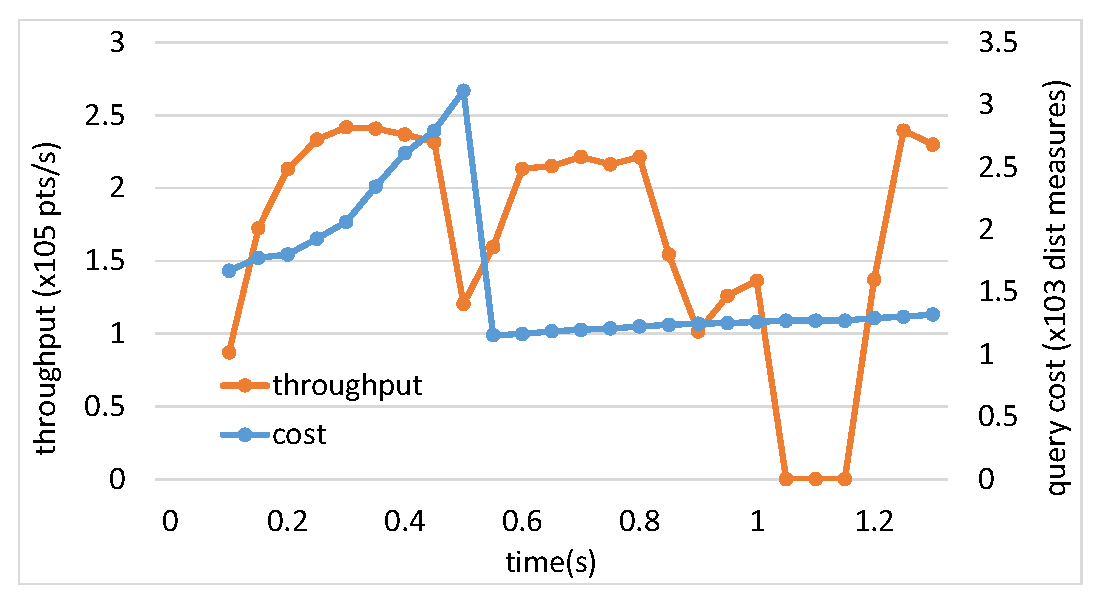
\includegraphics[width=2.6in]{fig/streaminsert.eps}}
    \vspace{-0.1in}
    \caption{The processing throughput and query cost for a sequence of insertions.}
    %\vspace{-0.1in}
    \label{fig:streaminsert}
\end{figure}

The processing throughput and query cost results are shown in Figure \ref{fig:streaminsert}. We can see that the processing throughput is obviously reduced after each time window (0.5s and 1s) since many overloaded buckets will be split at that time. Note that, the throughput may also drop within a time window since some buckets might be seriously overloaded (i.e., the bucket size is larger than $(1+\epsilon_m)\cdot T_u$) and cannot wait for the time window to end. The query cost for a specific point will be continuously increased until some of its host buckets are split. From this figure, this happens after the first time window (0.5s). It is probably because one of the query's host buckets is split. In addition, the throughput should be affected by $\epsilon_m$ and $\epsilon_c$. We run experiments and see that the throughput is increased when increasing $\epsilon_m$. For $\epsilon_m=(0.2,0.4,0.6,0.8,1)$, the average throughput results is $(1.25,1.49,1.66,1.77,2.28)\times 10^5$ pts/s.

\begin{comment}
\subsection{Distributed All-Pairs Computation}
\label{sec:expr:allpair}

In Section \ref{sec:distributed}, we introduce a use case of distributed all-pairs computation, i.e., point density evaluation. We conduct experiments to show the benefit of our proposed multi-layered LSH structure in distributed computing. The experiment is performed in a large distributed cluster which contains 64 m1.medium Amazon EC2 instances. Each instance is equipped with 1 vCPU, 3.75GB memory, and 410GB disk. We utilize LSH and LayerLSH to partition the BigCross dataset and approximate the point densities by using Hadoop MapReduce. The MapReduce implementation involves two jobs. The first performs LSH partition and all-pairs computation locally. The second job aggregates the local results. The LSH parameters are set as $l=3, m=3$. The expected accuracy is set to 0.95 such that $w$ can be computed based on Equation (\ref{eq:prob2}), since the radius for evaluating point density is given. In LayerLSH, the bucket size limit is set as 10000 rather than being set according to precision rate, since this is not a $k$NN query application. In addition, similar sparse buckets are merged to further improve accuracy and to reduce number of partitions. The lower bound of bucket size is set as 1000. The number of reduce tasks is set as 256.

\begin{figure}[t]
%\vspace{-0.1in}
    \centerline{\includegraphics[angle=-90, width=2in]{fig/amazon_buckets.eps}}
    %\vspace{-0.05in}
    \caption{The distribution of bucket size in LSH and LayerLSH (BigCross).}
    %\vspace{-0.2in}
    \label{fig:amazon_buckets}
\end{figure}

By applying LSH and LayerLSH, the bucket size distributions are depicted in Figure \ref{fig:amazon_buckets}. The dense buckets are rehashed and the sparse buckets are merged in LayerLSH, so that the skewed buckets are balanced. As known, workload balance is crucial for distributed computing, which could bring significant performance gain especially in a very large scale distributed environment.

\begin{figure}[t]
%\vspace{-0.1in}
	\centerline{
	\subfloat[LSH]{\includegraphics[angle=-90, width=1.8in]{fig/lshruntime.eps}
    \label{fig:amazon:lsh}
    \vspace{-0.05in}}
    \hspace{-5mm}
    \subfloat[LayerLSH]{\includegraphics[angle=-90, width=1.8in]{fig/layerlshruntime.eps}
    \label{fig:amazon:layerlsh}
    \vspace{-0.05in}}
    }
    %\vspace{-0.05in}
	\caption{The runtime of point density evaluation using Hadoop (BigCross).}
	\label{fig:amazon}
%\vspace{-0.2in}
\end{figure}

The runtime of reduce tasks are shown in Figure \ref{fig:amazon}. Each color bar represents a reduce task, which performs local all-pairs computation. Each worker is assigned with multiple reduce tasks. The skewed distribution of bucket sizes leads to the skewed runtime of reduce tasks. We can see that the runtime of reduce tasks is seriously skewed when using LSH. While the runtime of reduce tasks in LayerLSH is more balanced. Accordingly, LSH-based point density evaluation requires much longer runtime than LayerLSH-based approach (20h58m2s vs. 1h36m38s). Since the rehashing strategy of LayerLSH does not reduce accuracy and the sparse buckets are merged, the accuracy is even higher by using LayerLSH\footnote{Because we cannot obtain the exact density values of all points in a reasonable time, we only show the sum of density values. In terms of point density's definition, the larger density should be more accurate.}.
\end{comment}


